% !TeX spellcheck = en-GB
\section{Results}
A 5-fold cross validation yields a mean DICE of $0.91$ with a standard deviation of $0.03$. The range lies between $0.85$ and $0.96$ and has a median of $0.9$. In \autoref{fig:dicecrossvalid} the DICE after the prediction of the Random Forest is compared to the DICE after the post processing. One can see, that the post processing increases the results by $0.05$ on average. The average computation time for the whole proposed algorithm is $2.5$ minutes for one MRI volume. The goal of $0.95$ DICE is represented as the dashed line in \autoref{fig:dicecrossvalid}.
\begin{figure}[h]
\centering
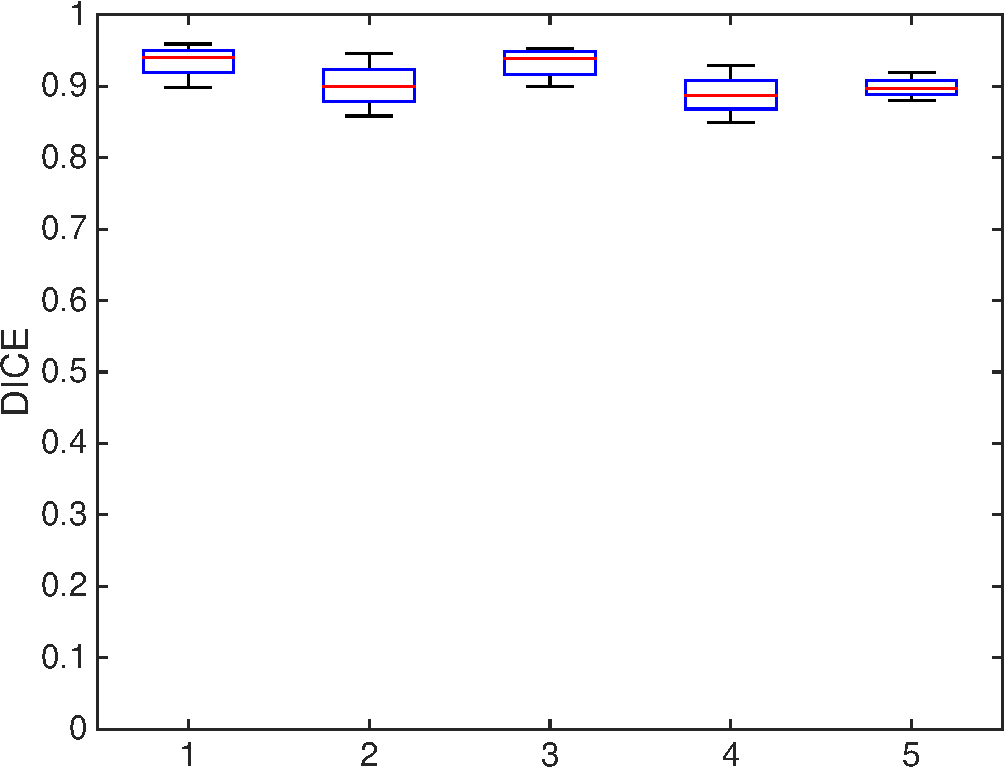
\includegraphics[width=\linewidth]{dicecrossvalid2.pdf}
\caption{The target DICE of $0.95$(dashed line) and the DICE yielded by the 5-fold cross validation on the first data set. The DICE is measured once after Random Forest and once after post processing.}
\label{fig:dicecrossvalid}
\end{figure}

In \autoref{fig:opjectiveResults} the optically best and worst result out of the second data set are shown. These are based on subjective observations and not on quantitative measurements, as the ground truth to this data is not available.
\begin{figure*}[!t]
	\centering
	\subfloat[Best case (image 29)]{
		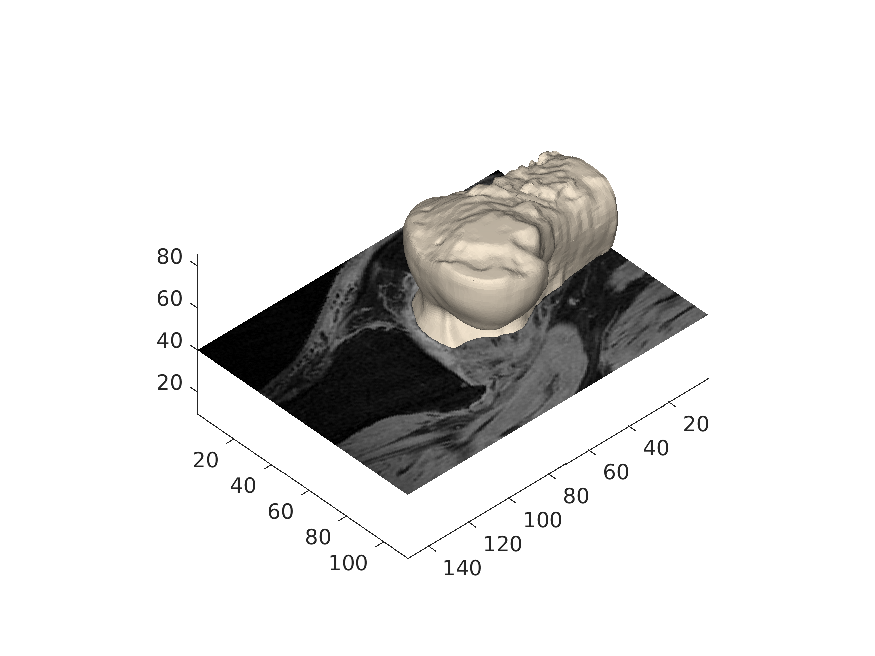
\includegraphics[width=0.48\textwidth]{vr029}
		\label{fig:bestcase}}
	\hfil
	\subfloat[Worst case (image 21)]{
		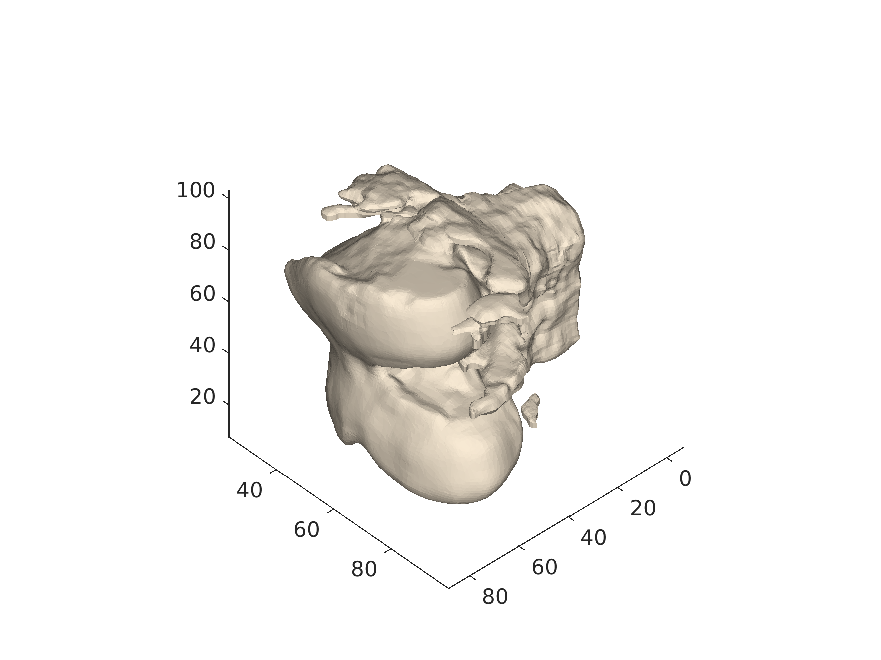
\includegraphics[width=0.48\textwidth]{vr021}
		\label{fig:worstcase}}
	
	\caption{Objectively the best and the worst segmentation of the second data set.}
	\label{fig:opjectiveResults}
\end{figure*}